\section{Durchführung}
\label{sec:Durchführung}

% Was wurde gemessen bzw. welche Größen wurden variiert?

\subsection{Aufname der Geiger-Müller Charakterisik}
\label{ssec:d1}

Für die Messungen wird eine Schaltung wie in \autoref{fig:aufbau} aufgebaut.
Auf dem Zähldraht im Geiger-Müller-Zählrohr sammelt sich die Ladung $Q$, diese fließt dann über den Widerstand $R$ ab und erzeugt eine Spannung.
Diese Spannung wird vom Kondensator $C$ ausgekoppelt und daraufhin verstärkt, damit sie dann im Zähler gemessen werden kann.


\begin{figure}
    \centering
    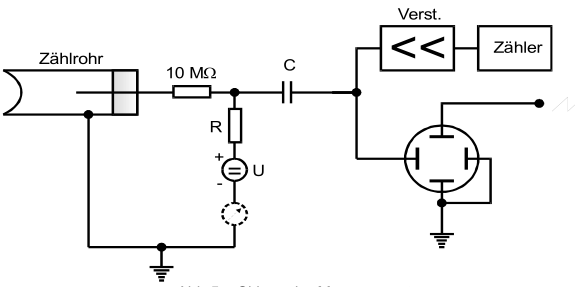
\includegraphics[width=\textwidth]{images/bild1.png}
    \caption{Aufbau der Messaperatur}
    \label{fig:aufbau}
\end{figure}

Nun wird eine Thallium-204-Quelle vor das Zählrohr gestellt, ein $\beta$ -Strahler.
Es ist wichtig zu beachten, dass alles so aufgebaut wird, dass die Zählrate nicht $\SI{100}{\text{Imps}\per\second}$ übersteigt.
Das wird getan, damit eine Totzeitkorrerkur nicht notwendig ist.
Die Zählrohrspannung $U$ wird auf $\SI{320}{\volt}$ gesetzt und es werden für je $\SI{60}{\second}$ die Impulse gemessen.
Dann wird die Spannung um $\SI{10}{\volt}$ vergrößert und erneut gemessen.
Dieser Vorgang wird bis einschließlich $\SI{700}{\volt}$ wiederholt.
Alle Daten werden notiert.

\subsection{Bestimmung der Totzeit}
\label{ssec:d2}

Um die gemessenen Impulse unter einer Totzeitkorrektur anspassen zu können muss zunächst der Wert für die Totzeit berechnet werden.
Zunächst wird die Thallium-204-Quelle näher an das Zählrohr gerückt, da die Intensität hoch genug steigen muss, damit eine Korrektur nötig wird.
Dann werden mit einer Integrationszeit von $\SI{120}{\second}$ die Impulse gemessen.
Zusätzlich wird eine zweite Quelle verwendet.
Für diese wird die gleiche Messung durchgeführt, wie für die erste.
Abschließend wird noch eine Messung mit beiden Quellen durchgeführt.
Wichtig ist, dass die Abstände der Quellen zum Zählrohr jeweils gleich bleiben, da es sonst die Messung verfälscht.
Die drei Werte für die Intensitäten werden notiert.

\subsection{Bestimmung der freigesetzten Ladungen pro Teilchen}
\label{ssec:d3}

Die Messung für diesen Teil kann ebneso zusammen mit \autoref{ssec:d1} durchgeführt werden.
Es muss lediglich ab $\SI{350}{\volt}$ an, alle $\SI{50}{\volt}$ die Stromstärke $I$ abgelesen werden.
Dabei hat das Amperemeter eine Ablesegenauigkeit von $\SI{0.05}{\micro\ampere}$.